\documentclass{beamer} 
\usepackage{amsmath,amsthm}
\usepackage{graphicx,microtype,parskip}
\usepackage{caption,subcaption,multirow}
\usepackage{attrib}

\frenchspacing

\usetheme{default}
\usecolortheme{whale}

\setbeamertemplate{navigation symbols}{}

\setbeamercolor{title}{fg=blue,bg=white}

\setbeamercolor{block title}{fg=white,bg=gray}
\setbeamercolor{block body}{fg=black,bg=lightgray}

\setbeamercolor{block title alerted}{fg=white,bg=darkgray}
\setbeamercolor{block body alerted}{fg=black,bg=lightgray}

\title{How do species traits affect extinction risk?}
\subtitle{New approaches to old questions.}
\author{Peter D Smits}
\institute{Committee on Evolutionary Biology}
\titlegraphic{
  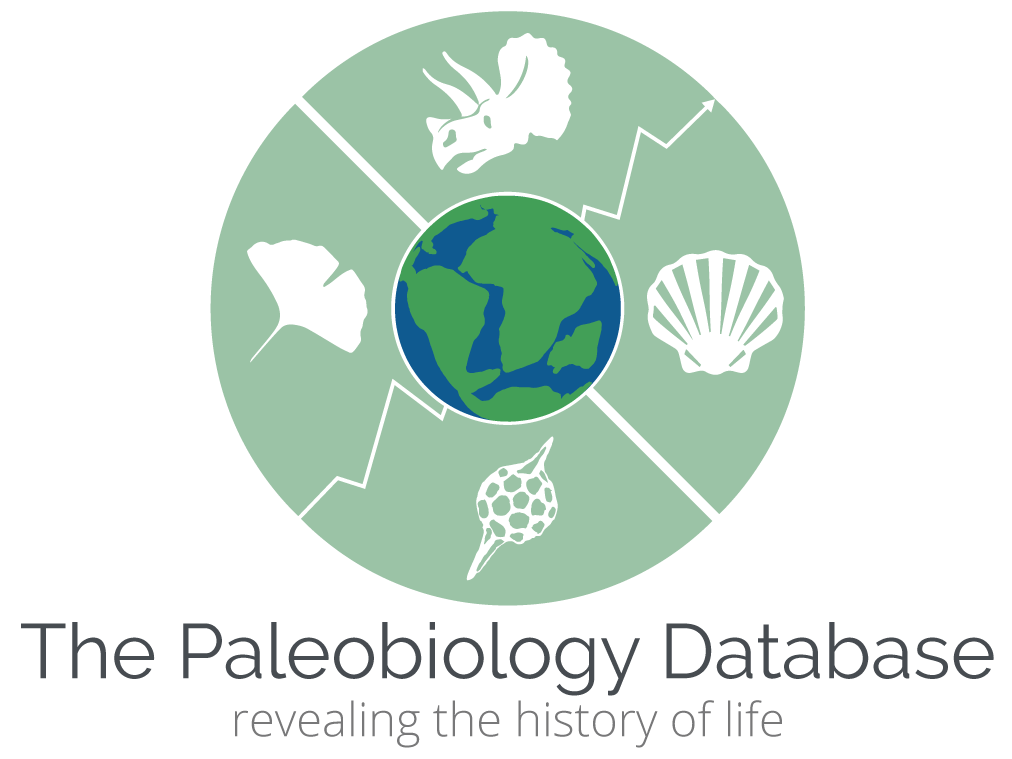
\includegraphics[width=2.75cm,height=2.75cm,keepaspectratio=true]{figure/paleodb}
  \hspace*{0.35\paperwidth}
  
\includegraphics[width=2cm,height=2cm,keepaspectratio=true]{figure/chicago}
}
\date{}

\begin{document}

\begin{frame}
  \titlepage
\end{frame}

\begin{frame}
  \begin{center}
    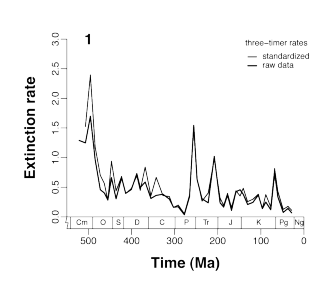
\includegraphics[width=0.5\textwidth,height=0.8\textheight,keepaspectratio=true]{figure/alroy_rates}
    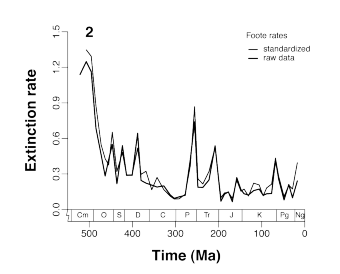
\includegraphics[width=0.5\textwidth,height=0.8\textheight,keepaspectratio=true]{figure/foote_rates}
  \end{center}
\end{frame}

\begin{frame}
  \begin{alertblock}{Question}
    Why do taxa go extinct at different rates?
  \end{alertblock}
\end{frame}



% example studies
%   time-invariant differences in mammal species durations
\begin{frame}
  \frametitle{Two studies}
  \begin{columns}
    \begin{column}{0.5\textwidth}
      \begin{center}
        \textbf{Brachiopods}

        \vspace{0.5cm}

        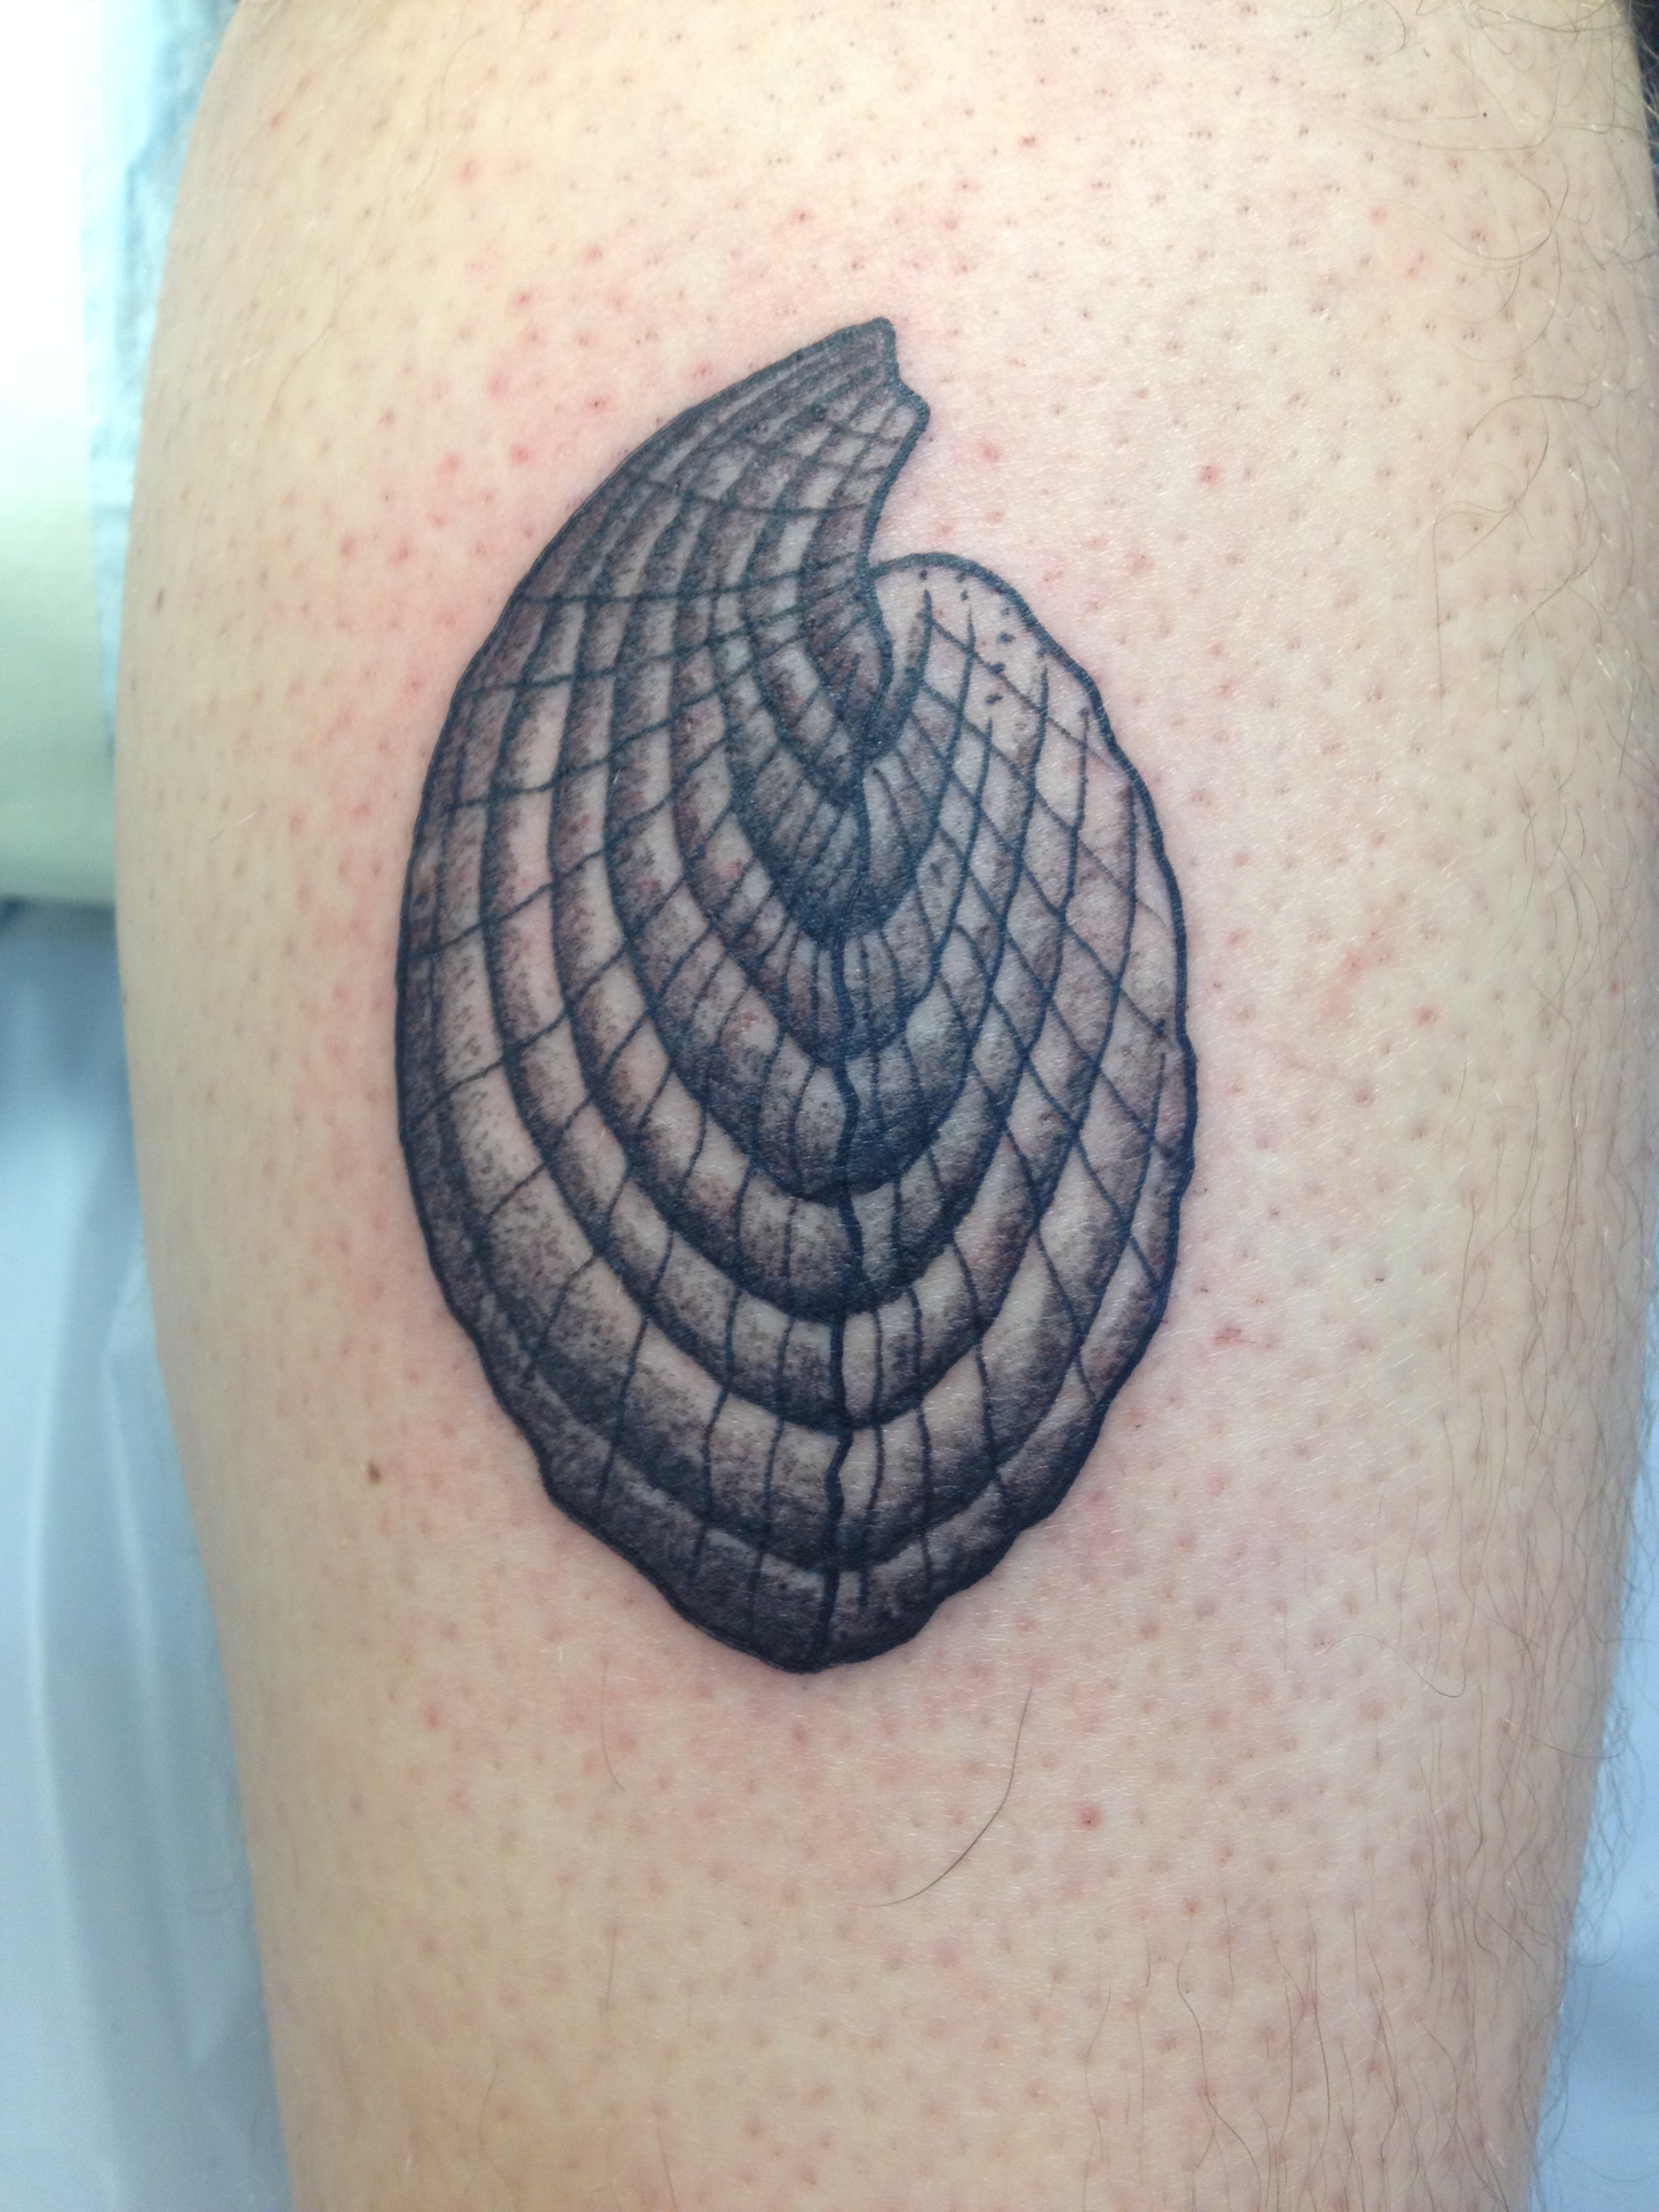
\includegraphics[height = 0.4\textheight, keepaspectratio = true]{figure/tattoo}
      \end{center}
    \end{column}
    \begin{column}{0.5\textwidth}
      \begin{center}
        \textbf{Mammals}

        \vspace{0.5cm}

        
\includegraphics[height = 0.4\textheight, keepaspectratio = true]{figure/annyong}
      \end{center}
    \end{column}
  \end{columns}
\end{frame}

% my approach
%   survival analysis
%     S(t)
%     exponential vs weibull
%   hierarchical Bayesian modelling
\begin{frame}
  \frametitle{First things first\dots}

  \begin{block}{(Some) notational definitions to help navigate}
    \begin{itemize}
      \item \(y_{i}\): duration of taxon \(i\)
      \item \(\mathbf{X}\): \(n \times k\) matrix of covariates
      \item \(\sim\): rhs stochastically distributed as lhs
      \item \(\beta\): regression coefficient
      \item \(j[i]\): taxon \(i\) belongs to group \(j\)
    \end{itemize}
  \end{block}
\end{frame}

\begin{frame}
  \frametitle{Study: mammal species duration}
  \begin{alertblock}{Questions}
    \begin{itemize}
      \item How do the covariates of interest affect extinction risk?
      \item What is the relative contribution of temporal and phylogenetic structure on extinction risk?
      \item How do the identified time-invariant effects compare to modern determinates of extinction risk?
    \end{itemize}
  \end{alertblock}
\end{frame}
  % data
  %   North America
  %   Cenozoic
  %   PBDB
  % covariates of interest
  %   dietary category
  %   locomotor category
  %   body size
  %   bioprovince occupancy
  % structure
  %   non-nested varying intercepts
  %   origination cohort \(j\)
  %   phylogenetic position of \(i\)

\begin{frame}
  \frametitle{Model of mammal species survival}
  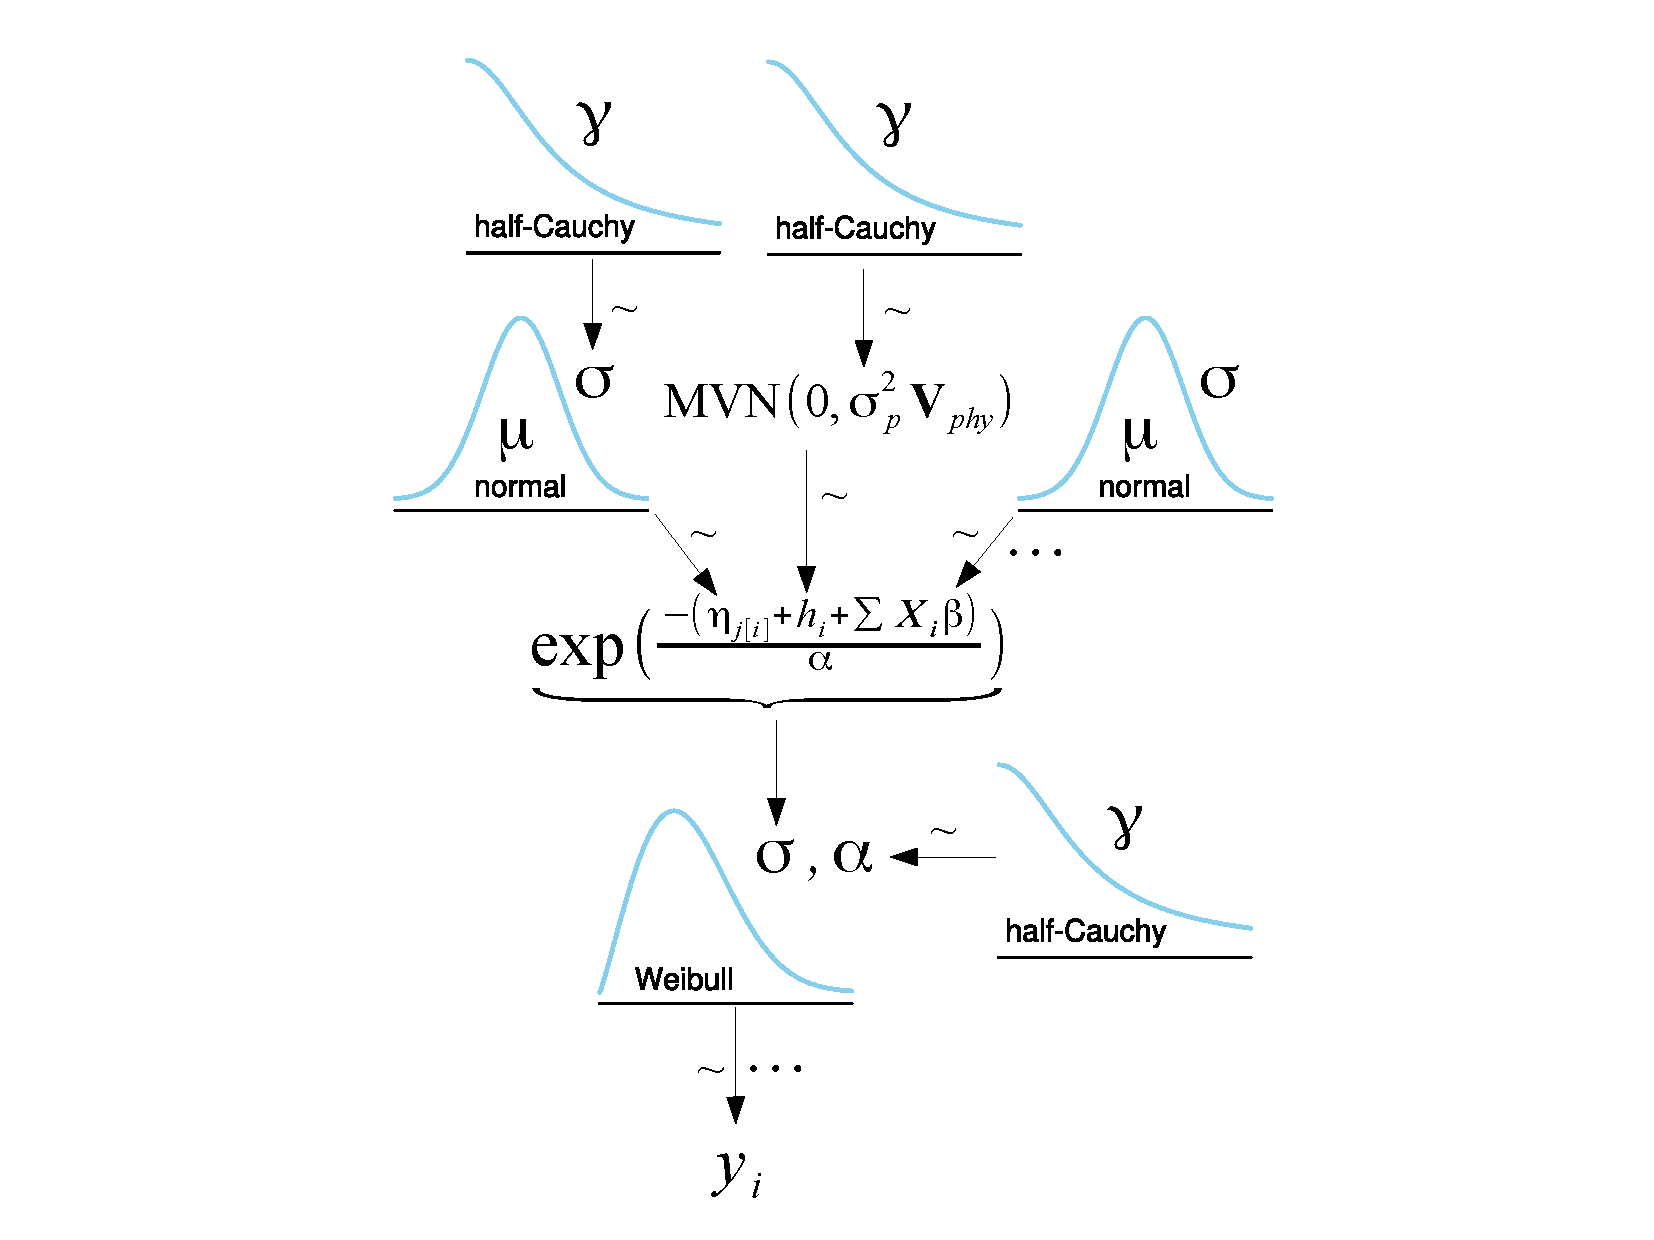
\includegraphics[width=\textwidth,height=0.8\textheight,keepaspectratio=true]{figure/mammal_survival_model}
\end{frame}


%   *brachiopods*
\begin{frame}
  \frametitle{Study: brachiopod genus duration}
  \begin{alertblock}{Questions}
    \begin{itemize}
      \item How do the covariates of interest affect extinction risk?
      \item How do these trait-based effects vary between origination cohorts?
      \item How do these trait-based changes relate to changes in baseline extinction risk?
    \end{itemize}
  \end{alertblock}
\end{frame}
  % data
  %   Global
  %   Paleozoic
  %   PBDB (Foote/Miller)
  % covariates of interest
  %   geographic range size
  %   environmental affinity
  %   body size
  % structure
  %   varying intercepts, varying slopes
  %   origination cohort \(j\)

\begin{frame}
  \frametitle{Model of brachiopod genus survival}
  \begin{align*}
    y_{i} &\sim \mathrm{Weibull}(\alpha, \sigma) \\
    \sigma_{i} &= \exp\left(\frac{-(\mathbf{X}_{i} \mathbf{B}_{j[i]})}{\alpha}\right) \\
    \mathbf{B} &\sim \mathrm{MVN}(\vec{\mu}, \mathbf{\Sigma}) \\
    \mathbf{\Sigma} &= \text{Diag}(\vec{\tau}) \mathbf{\Omega} \text{Diag}(\vec{\tau}) \\
    \alpha &\sim \mathrm{C^{+}}(2) \\
    \mu_{\kappa} &\sim \mathcal{N}(0, 5) \text{ for } \kappa \in 1:k \\
    \tau_{\kappa} &\sim \mathrm{C^{+}}(1) \text{ for } \kappa \in 1:k \\
    \mathbf{\Omega} &\sim \text{LKJ}(2).
  \end{align*}

  \bigskip

  \footnotesize{Unreadable. I know.}
\end{frame}


% summary
%   survival of the unspecialized
%
%   time-invariant differences in Cenozoic mammal survival qualitatively different from modern determinates of extinction risk
%
%   negative correlation between baseline extinction and effect of traits (except for geographic range)
\begin{frame}
  \frametitle{Summary}
\end{frame}

% acknowledgements
%   committee
%   data sources
%   discussion
\begin{frame}
  \frametitle{Acknowledgements}
\end{frame}


\end{document}
